\documentclass[a4paper, 11pt]{article}
\usepackage[UTF8, scheme = plain]{ctex}
\usepackage{float}
\usepackage{amsmath}
\usepackage{graphicx}
\usepackage{geometry}
\usepackage{listings}
\geometry{scale=0.8}
\linespread{1.5}
\usepackage{hyperref}

\title{	
\normalfont \normalsize
\textsc{School of Data and Computer Science, Sun Yat-sen University} \\ [25pt] %textsc small capital letters
\rule{\textwidth}{0.5pt} \\[0.4cm] % Thin top horizontal rule
\huge  E08 FF Planner(2)\\ % The assignment title
\rule{\textwidth}{2pt} \\[0.5cm] % Thick bottom horizontal rule
\author{20214966 Yangkai Lin 20214810 Suixin Ou}
\date{\normalsize\today}
}

\begin{document}
\maketitle
\tableofcontents
\newpage
\section{Boxman Game}
If you don't know how to play the boxman game, you should open \texttt{BoxMan.zip} and click \texttt{BoxMan.exe} to have a try.  You can also choose the level of the game to challenge yourselves. There are five cases choosed from level 1, 10, 30, 40, 50 in the following figures.

You can model the location information based on rectangular coordinates as mapped out in Figure 3. For example, we denote by P13 the position (1,3). The calculated action sequence can be like this: \texttt{MOVE P12 P13, PUSH BOX1 P14 P15...},which means the guy runs from position (1,2) to position (1,3), and push the box1 from position (1,4) to position (1,5). However, this is only a very simple and intuitive approach to representing the actions and positions. If you have any other better methods, you can have a try.

Please solve the boxman game by using FF planner. You should hand in 2 files, including a domain file (\texttt{boxman\_domain.pddl}) and  data file (\texttt{boxman5.pddl}).
\begin{figure}[H]
  \centering
  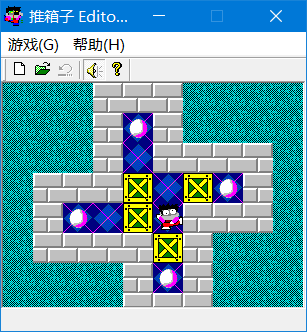
\includegraphics[width=6cm]{Pic/case1}
  \qquad
  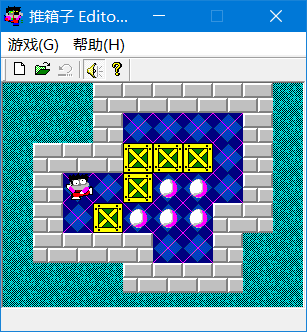
\includegraphics[width=6cm]{Pic/case2}
  \caption{Boxman case1 (level 1) and case2 (level 10)}
\end{figure}
\begin{figure}[H]
  \centering
  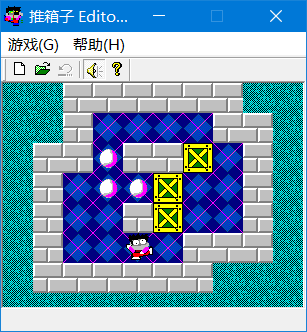
\includegraphics[width=6cm]{Pic/case3}
  \qquad
  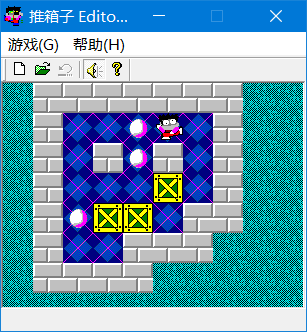
\includegraphics[width=6cm]{Pic/case4}
  \caption{Boxman case3 (level 30) and case4 (level 40)}
\end{figure}
\begin{figure}[H]
  \centering
  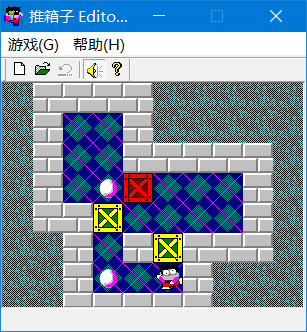
\includegraphics[width=6cm]{Pic/case5}
  \qquad
  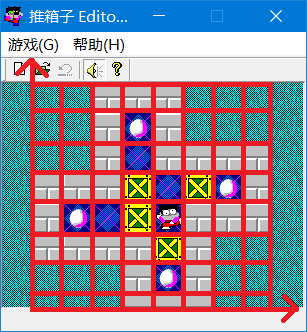
\includegraphics[width=6cm]{Pic/model}
  \caption{Boxman case5 (level 50) and modelling}
\end{figure}


\section{Codes}
\subsection{域实现}
\subsubsection{定义predicates}
\begin{itemize}
\item\textit{blank(p)}: 位置p无人也无箱子。
\item\textit{man(p)}: 位置p有人。
\item\textit{at(b,p)}: 箱子x在位置p。
\item\textit{line(p0,p1,p2)}: 位置p0,p1,p2连成一条线。
\item\textit{adjacent(p1,p2)}: 位置p1,p2相邻。
\end{itemize}
\subsubsection{boxman\_domain.pddl}
\begin{lstlisting}[title=boxman\_domain.pddl,frame=single,language=lisp,numbers=left]
(define (domain boxman)
  (:requirements :strips :typing:equality
                  :universal-preconditions
                  :negative-preconditions)
  (:types box loc)
  (:predicates
    (blank ?p - loc)
    (man ?p - loc)
    (at ?b - box ?p - loc)
    (line ?p0 ?p1 ?p2 -loc)
    (adjacent ?p1 ?p2 -loc)
  )   

  (:action move
    :parameters (?from ?to - loc)
    :precondition (and (man ?from) (blank ?to) (adjacent ?from ?to))
    :effect (and (not (man ?from)) (not (blank ?to))
                  (man ?to) (blank ?from))
  )

  (:action push
    :parameters (?box - box ?p1 ?p2 ?p3 - loc)
    :precondition (and (man ?p1) (at ?box ?p2) (blank ?p3)
                        (line ?p1 ?p2 ?p3))
    :effect (and (not (man ?p1)) (not (at ?box ?p2)) (not (blank ?p3))
                  (man ?p2) (at ?box ?p3) (blank ?p1))
  )
)
\end{lstlisting}
\subsection{初始状态和目标实现}
\subsubsection{初始化adjacent(p1,p2)和line(p0,p1,p2)}
考虑两点相邻即两点曼哈顿距离为1。
\begin{lstlisting}[title=adjacent.py,frame=single,language=python,numbers=left]
l = ['P32',
     'P42',
     'P52',
     'P33',
     'P53',
     'P34',
     'P44',
     'P54',
     'P64',
     'P74',
     'P25',
     'P35',
     'P45',
     'P55',
     'P65',
     'P75',
     'P26',
     'P36',
     'P27',
     'P37']
for pos1 in l:
    for pos2 in l:
        if abs(int(pos1[1]) - int(pos2[1]))\
        + abs(int(pos1[2]) - int(pos2[2])) == 1:
            print('(adjacent ' + pos1 + ' ' + pos2 + ')')
\end{lstlisting}
考虑三点共线,即$(x_1-x_2)\cdot(x_2-x_3)=1$且$y_1=y_2=y_3$
或$(y_1-y_2)\cdot(y_2-y_3)=1$且$x_1=x_2=x_3$。
\begin{lstlisting}[title=line.py,frame=single,language=python,numbers=left]
l = ['P32',
     'P42',
     'P52',
     'P33',
     'P53',
     'P34',
     'P44',
     'P54',
     'P64',
     'P74',
     'P25',
     'P35',
     'P45',
     'P55',
     'P65',
     'P75',
     'P26',
     'P36',
     'P27',
     'P37']
for pos1 in l:
    for pos2 in l:
        for pos3 in l:
            if (int(pos1[1]) - int(pos2[1]))\
            * (int(pos2[1]) - int(pos3[1])) == 1\
                and pos1[2] == pos2[2] and pos2[2] == pos3[2]:
                    print('(line ' + pos1 + ' '\
                        + pos2 + ' ' + pos3 + ')')
            elif (int(pos1[2]) - int(pos2[2]))\
            * (int(pos2[2]) - int(pos3[2])) == 1\
                and pos1[1] == pos2[1] and pos2[1] == pos3[1]:
                    print('(line ' + pos1 + ' '\
                        + pos2 + ' ' + pos3 + ')')
\end{lstlisting}
\subsubsection{boxman.pddl}
\begin{lstlisting}[title=boxman.pddl,frame=single,language=lisp,numbers=left]
(define (problem prob)
    (:domain boxman)
    (:objects BOX1 BOX2 BOX3 - box
        P32 P42 P52 P33 P53 P34 P44 P54 P64 P74
        P25 P35 P45 P55 P65 P75 P26 P36 P27 P37 - loc)
    (:init
        (adjacent P32 P42)
        (adjacent P32 P33)
        (adjacent P42 P32)
        (adjacent P42 P52)
        (adjacent P52 P42)
        (adjacent P52 P53)
        (adjacent P33 P32)
        (adjacent P33 P34)
        (adjacent P53 P52)
        (adjacent P53 P54)
        (adjacent P34 P33)
        (adjacent P34 P44)
        (adjacent P34 P35)
        (adjacent P44 P34)
        (adjacent P44 P54)
        (adjacent P44 P45)
        (adjacent P54 P53)
        (adjacent P54 P44)
        (adjacent P54 P64)
        (adjacent P54 P55)
        (adjacent P64 P54)
        (adjacent P64 P74)
        (adjacent P64 P65)
        (adjacent P74 P64)
        (adjacent P74 P75)
        (adjacent P25 P35)
        (adjacent P25 P26)
        (adjacent P35 P34)
        (adjacent P35 P25)
        (adjacent P35 P45)
        (adjacent P35 P36)
        (adjacent P45 P44)
        (adjacent P45 P35)
        (adjacent P45 P55)
        (adjacent P55 P54)
        (adjacent P55 P45)
        (adjacent P55 P65)
        (adjacent P65 P64)
        (adjacent P65 P55)
        (adjacent P65 P75)
        (adjacent P75 P74)
        (adjacent P75 P65)
        (adjacent P26 P25)
        (adjacent P26 P36)
        (adjacent P26 P27)
        (adjacent P36 P35)
        (adjacent P36 P26)
        (adjacent P36 P37)
        (adjacent P27 P26)
        (adjacent P27 P37)
        (adjacent P37 P36)
        (adjacent P37 P27)
        (line P32 P42 P52)
        (line P32 P33 P34)
        (line P52 P42 P32)
        (line P52 P53 P54)
        (line P33 P34 P35)
        (line P53 P54 P55)
        (line P34 P33 P32)
        (line P34 P44 P54)
        (line P34 P35 P36)
        (line P44 P54 P64)
        (line P54 P53 P52)
        (line P54 P44 P34)
        (line P54 P64 P74)
        (line P64 P54 P44)
        (line P74 P64 P54)
        (line P25 P35 P45)
        (line P25 P26 P27)
        (line P35 P34 P33)
        (line P35 P45 P55)
        (line P35 P36 P37)
        (line P45 P35 P25)
        (line P45 P55 P65)
        (line P55 P54 P53)
        (line P55 P45 P35)
        (line P55 P65 P75)
        (line P65 P55 P45)
        (line P75 P65 P55)
        (line P36 P35 P34)
        (line P27 P26 P25)
        (line P37 P36 P35)
        (man P52)
        (at BOX1 P53)
        (at BOX2 P34)
        (at BOX3 P45)
        (blank P32)
        (blank P42)
        (blank P33)
        (blank P44)
        (blank P54)
        (blank P64)
        (blank P74)
        (blank P25)
        (blank P35)
        (blank P55)
        (blank P65)
        (blank P75)
        (blank P26)
        (blank P36)
        (blank P27)
        (blank P37)
    )
    (:goal (and (and (not (blank P32)) (not (man P32)))
                (and (not (blank P35)) (not (man P35)))
                (and (not (blank P45)) (not (man P45)))))
)
\end{lstlisting}

\section{result}
\begin{lstlisting}[title=result.txt,frame=single,basicstyle=\tiny]
Planning service: http://solver.planning.domains/solve
Domain: boxman, Problem: prob
 --- OK.
 Match tree built with 110 nodes.

PDDL problem description loaded: 
	Domain: BOXMAN
	Problem: PROB
	#Actions: 110
	#Fluents: 119
Landmarks found: 6
Starting search with IW (time budget is 60 secs)...
rel_plan size: 6
#RP_fluents 23
Caption
{#goals, #UNnachieved,  #Achieved} -> IW(max_w)

{6/3/0}:IW(1) -> rel_plan size: 6
#RP_fluents 23
{6/3/2}:IW(1) -> rel_plan size: 6
#RP_fluents 23
{6/2/3}:IW(1) -> [2][3][4][5]rel_plan size: 2
#RP_fluents 8
{6/1/4}:IW(1) -> [2][3][4][5][6][7][8][9][10];; NOT I-REACHABLE ;;
Total time: 0.004
Nodes generated during search: 87
Nodes expanded during search: 75
IW search completed
Starting search with BFS(novel,land,h_add)...
--[4294967295 / 6]--
--[2 / 6]--
--[2 / 4]--
--[2 / 3]--
--[2 / 2]--
--[2 / 1]--
--[1 / 1]--
--[1 / 0]--
--[0 / 0]--
Total time: 0.572
Nodes generated during search: 20099
Nodes expanded during search: 8026
Plan found with cost: 51
BFS search completed
0.00100: (push box1 p52 p53 p54)
0.00200: (move p53 p52)
0.00300: (move p52 p42)
0.00400: (move p42 p32)
0.00500: (move p32 p33)
0.00600: (push box2 p33 p34 p35)
0.00700: (move p34 p44)
0.00800: (push box1 p44 p54 p64)
0.00900: (move p54 p55)
0.01000: (move p55 p65)
0.01100: (move p65 p75)
0.01200: (move p75 p74)
0.01300: (push box1 p74 p64 p54)
0.01400: (push box1 p64 p54 p44)
0.01500: (move p54 p53)
0.01600: (move p53 p52)
0.01700: (move p52 p42)
0.01800: (move p42 p32)
0.01900: (move p32 p33)
0.02000: (move p33 p34)
0.02100: (push box2 p34 p35 p36)
0.02200: (push box3 p35 p45 p55)
0.02300: (push box3 p45 p55 p65)
0.02400: (move p55 p54)
0.02500: (push box1 p54 p44 p34)
0.02600: (move p44 p45)
0.02700: (move p45 p35)
0.02800: (push box1 p35 p34 p33)
0.02900: (push box1 p34 p33 p32)
0.03000: (move p33 p34)
0.03100: (move p34 p35)
0.03200: (move p35 p25)
0.03300: (move p25 p26)
0.03400: (move p26 p27)
0.03500: (move p27 p37)
0.03600: (push box2 p37 p36 p35)
0.03700: (move p36 p26)
0.03800: (move p26 p25)
0.03900: (push box2 p25 p35 p45)
0.04000: (move p35 p34)
0.04100: (move p34 p44)
0.04200: (move p44 p54)
0.04300: (move p54 p55)
0.04400: (push box2 p55 p45 p35)
0.04500: (move p45 p55)
0.04600: (move p55 p54)
0.04700: (move p54 p64)
0.04800: (move p64 p74)
0.04900: (move p74 p75)
0.05000: (push box3 p75 p65 p55)
0.05100: (push box3 p65 p55 p45)
Planner found 1 plan(s) in 1.567secs.
\end{lstlisting}


\section{Notes}


\par Please send \textbf{E08\_YourNumber.zip} which should contain the codes(\textbf{ai\_2020@foxmail.com}). 




%\clearpage
%\bibliography{E:/Papers/LiuLab}
%\bibliographystyle{apalike}
\end{document} 
%%% Local Variables:
%%% mode: latex
%%% TeX-master: t
%%% End:
